
\chapter[Reaching Definitions Analyzer for C Programs]{Reaching Definitions Analyzer for C Programs}
\label{ch:lab6} % This how you label a chapter and the key (e.g., ch:into) will be used to refer this chapter ``Introduction'' later in the report. 
% the key ``ch:into'' can be used with command \ref{ch:intor} to refere this Chapter.

\begin{center}
    \href{https://github.com/jsmaskeen/CS202-STTCSE/tree/lab7}{Github Repository for Lab 7}
\end{center}

\section{Introduction}
In this lab we implement a Reaching Definitions Analyzer for C programs from
scratch. We create our own custom simple parser, conver the C code into a
parsed tree, then make a control flow graph from it by identifying basic blocks
and their connections. Finally, we implement the reaching definitions analysis
using the iterative algorithm discussed in class. Reaching Definitions Analysis
is a fundamental data-flow analysis technique used in compilers to determine
which definitions (assignments of values to variables) may reach a given point
in the program. This is useful for optimizations such as dead code elimination
and, constant propagation etc. We use an example of simple C program to
illustrate the steps and output of our analysis. We run the analysis on three
non-trivial C programs (200-300 LOC) and store their results on the Github
repository for this lab.

\section{Setup and Tools}
We have Python, and VSCode installed. \texttt{python {-}{-}version} gives
\texttt{Python 3.12.4} as the output. The operating system on which all
commands and analysis are performed is Windows 11. We use \textbf{Graphviz} to
visualize the control flow graphs, and matplotlib to plot graphs for other
metrics. The Python packages used are \texttt{graphviz}, \texttt{matplotlib},
and \texttt{pandas}. These can be installed via pip. \texttt{dot --version}
gives \texttt{dot - graphviz version 13.1.0 (20250701.0955)} as the output.

\begin{figure}[!ht]
    \centering
    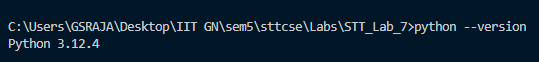
\includegraphics[width=0.5\linewidth]{figures/2_1.png}
    \caption{Python Version}
    \label{2_1}
\end{figure}
The working directory is named \texttt{STT\_Lab\_7}.

\section{Methodology and Execution}

\subsection{Program Selection}
We use four C programs for our analysis. They are as follows:
\begin{enumerate}
    \item \texttt{dft.c} (291 LOC): A program that implements the Discrete Fourier Transform. This program was chosen for its use of loops and arrays.
    \item \texttt{integration.c} (250 LOC): A program that performs numerical integration along with other computations such as computing $\pi$. This program was selected for its mathematical computations, calling external procedures (considered as blackbox) and more complex control flow.
    \item \texttt{labyrinth\_game.c} (460 LOC): A simple game that navigates a labyrinth. This program was chosen for its interactive nature and its use of nested loops and conditionals.
    \item \texttt{simple.c}: A basic program with conditional statements and variable reassignments. This program is used to provide a clear, step-by-step walkthrough of the analysis process.
\end{enumerate}
All programs are standalone \texttt{.c} files with a \texttt{main()} function, and the analysis is intraprocedural.

We make sure that all our programs do not have \texttt{goto} statements or
\texttt{break} or \texttt{switch} statemets, as to keep the parsing and
analysis simpler. Function calls to external procedures are treated as black
boxes. We also ensure that the code is formatted using
\url{https://marketplace.visualstudio.com/items?itemName=ms-vscode.cpptools}
extension in VSCode.

Throughout the parsing part, we utilise heavy regular expressions to identify
various constructs in the C code. We explain the entire process of parsing and
analysis using the simple.c program, which is as follows:

Initial C code:
\begin{lstlisting}[language=C]
#include <stdio.h>

int random_procedure()
{
    return 23;
}

int main(void)
{
    int i = 0;
    int x = 5;
    int y = -1;

    while (i < 10)
    {
        i = i + 1;
        y = i + x;
        printf("%d", i);
        if (i > 5)
        {
            x = i;
            printf("more than 5");
        }
    }

    random_procedure();

    for (int j = 0; j < 5; j++)
    {
        int z = j + y;
        printf("%d", z);
        random_procedure();
    }
    return 0;
}
\end{lstlisting}

\subsection{Parsing the C Code}
The first step is to extract out the main function and remove blank lines and
split at each newline character. This is how the program looks after this step:
\begin{lstlisting}[language=Python]
['int i = 0;',
 'int x = 5;',
 'int y = -1;',
 'while (i < 10)',
 '{',
 'i=i+1;',
 'y = i + x;',
 'printf("%d", i);',
 'if (i > 5)',
 '{',
 'x = i;',
 'printf("more than 5");',
 '}',
 '}',
 'random_procedure();',
 'for (int j = 0; j < 5; j++)',
 '{',
 'int z = j + y;',
 'printf("%d", z);',
 'random_procedure();',
 '}',
 'return 0;']
\end{lstlisting}

Now, we convert this into a nested structure (Equivalent to a very rudimentary
AST) using a recursive function. We identify blocks using curly braces, and
each block is represented as a list of statements. Each statement can be a
simple statement (like an assignment or a function call) or a control structure
(like if, while, for) which contains its own nested list of statements. The
resulting structure looks like this:

\begin{lstlisting}[language=Python]
[{'code': 'int i = 0;', 'type': 'statement'},
 {'code': 'int x = 5;', 'type': 'statement'},
 {'code': 'int y = -1;', 'type': 'statement'},
 {'body': [{'code': 'i=i+1;', 'type': 'statement'},
           {'code': 'y = i + x;', 'type': 'statement'},
           {'code': 'printf("%d", i);', 'type': 'statement'},
           {'body': [{'code': 'x = i;', 'type': 'statement'},
                     {'code': 'printf("more than 5");', 'type': 'statement'}],
            'condition': 'i > 5',
            'type': 'if'}],
  'condition': 'i < 10',
  'loop_type': 'while',
  'type': 'loop'},
 {'code': 'random_procedure();', 'type': 'statement'},
 {'body': [{'code': 'int z = j + y;', 'type': 'statement'},
           {'code': 'printf("%d", z);', 'type': 'statement'},
           {'code': 'random_procedure();', 'type': 'statement'}],
  'condition': 'j < 5',
  'increment': 'j++',
  'initialization': 'int j = 0',
  'loop_type': 'for',
  'type': 'loop'},
 {'code': 'return 0;', 'type': 'statement'}]
\end{lstlisting}

With this, we proceed to Control Flow Graph (CFG) generation.

\subsection{Control Flow Graph Generation}
A CFG is a directed graph where each node is a basic block (a sequence of
instructions with one entry and one exit) and each edge shows a possible
transfer of control (normal fall-through, true/false branch, loop-back, etc.).

We define two classes, \texttt{BasicBlock} and \texttt{ControlFlowGraph}. The
\texttt{BasicBlock} class represents a basic block with its statements and
successors. The \texttt{ControlFlowGraph} class manages the collection of basic
blocks and the start block, and a few other helper variables for Reaching
Defintions Analysis.\\ \noindent Note: In the following procedure, we refer to
the CFG class as \textit{builder}.

Using the following way, the above rudimentary AST is converted into a CFG:

\begin{enumerate}
    \item Entry and statements:
          \begin{itemize}
              \item The first call creates B0 (start). Every plain statement (type "statement") is
                    appended to the current block's instructions.
              \item If a statement appears where a new block should start, a new BasicBlock is
                    created and linked from the previous block.
          \end{itemize}
    \item If statements:
          \begin{itemize}
              \item The builder places the \texttt{if (cond)} as an instruction in the current
                    block.
              \item Then it creates a new block for the if-body and adds an edge from the if-block
                    to that body with label "true".
              \item It also creates an after-if block (the join). The last block of the if-body is
                    connected to the after-if block.
              \item If there is an else statement, an else block is created and connected with label
                    "false", and its last block also goes to the join. If no else is present, the
                    builder creates a "false" edge from the if-block to the join directly.
              \item Execution continues at the after-if block.
          \end{itemize}

    \item Loop statements:
          \begin{itemize*}
              \item For loop:
                    \begin{itemize}
                        \item If an initialization exists, it is used as an instruction in the current block
                              (Eg. \texttt{int j = 0;})
                        \item A condition block is created that contains \texttt{if (condition)} and has two
                              outgoing edges: "true" to the loop body and "false" to after-loop.
                        \item The loop body is a separate block; after the body, control goes to an increment
                              block (which contains the increment code, if any), and the increment block
                              links back to the condition block.
                    \end{itemize}
              \item While loop:
                    \begin{itemize}
                        \item The builder places the \texttt{while (cond)} as an instruction in the current
                              block (the block acts like a condition node).
                        \item The "true" edge goes to the loop body; when the body finishes it links back to
                              the condition block.
                        \item The "false" edge goes to the after-loop block.
                    \end{itemize}
          \end{itemize*}
\end{enumerate}

The exporting of the CFG is handled separately, where each node label contains
the block name plus its instructions (the code statements). The edges include
optional labels like "true" / "false" (Fig.~\ref{2_2}). The dot file is saved
then rendered using the dot CLI (Fig.~\ref{2_3}).

\begin{figure}[!ht]
    \centering
    \begin{minipage}{0.49\linewidth}
        \centering
        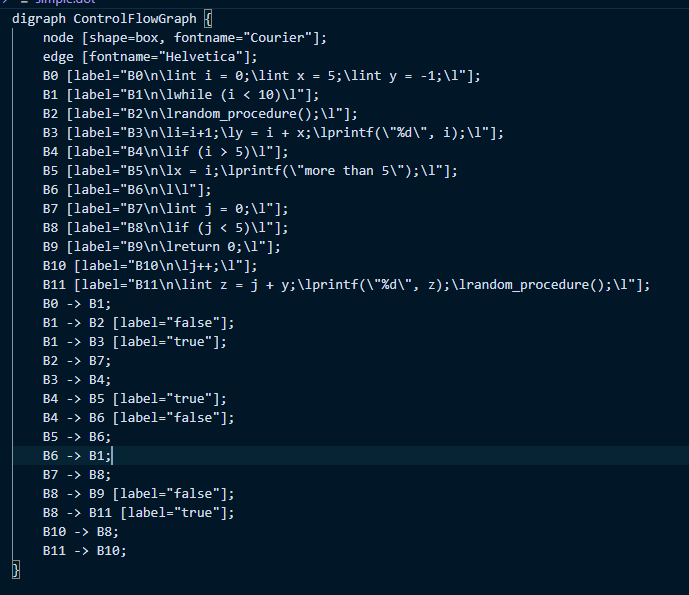
\includegraphics[width=\linewidth]{figures/2_2.png}
        \caption{Dot File for the CFG of simple.c}
        \label{2_2}
    \end{minipage}
    \hfill
    \begin{minipage}{0.49\linewidth}
        \centering
        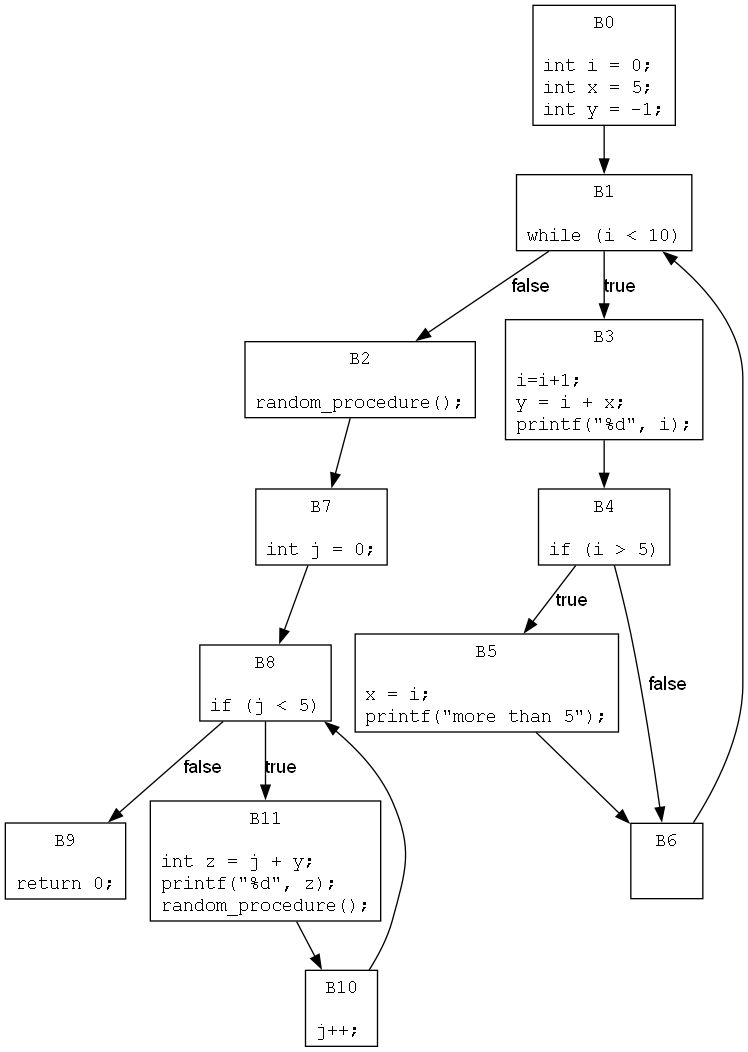
\includegraphics[width=\linewidth]{figures/2_3.png}
        \caption{Rendered dot File for the CFG of simple.c}
        \label{2_3}
    \end{minipage}
\end{figure}

\subsection{Cyclomatic Complexity Calculation}
After constructing the CFG, we compute the cyclomatic complexity of the
program. Cyclomatic complexity is a metric used to indicate the complexity of a
program. It is the number of independent paths through a program's source code.
It is calculated using the formula (for a single component):
\[ E-N+2 \]
where, E is the number of edges in the graph, and N is the number of nodes in
the graph. For the simple.c program, E=14, N=12, giving a cyclomatic complexity
of 4.

\subsection{Reaching Definitions Analysis}
Reaching Definitions Analysis determins, for each point in the program, which
definitions (assignments of values to variables) can reach that point. The
program points are the entry or exit of each basic block in the CFG.

The dataflow equations for Reaching Definitions Analysis are as follows:

\[
    in[B] = \union_{P \in pred(B)} out[P]
\]
\[out[B] = gen[B] \cup (in[B] - kill[B])
\]
Where:
\begin{itemize}
    \item \(in[B]\) is the set of definitions reaching the entry of block B.
    \item \(out[B]\) is the set of definitions reaching the exit of block B.
    \item \(gen[B]\) is the set of definitions generated within block B.
    \item \(kill[B]\) is the set of definitions that are killed (overwritten) by block B.
    \item \(pred(B)\) is the set of predecessor blocks of B in the CFG.
\end{itemize}
These equations are applied iteratively until the in and out sets converge (i.e., they no longer change).
Initially, all in[B] sets and out[B] sets are initialized to $\phi$.

The result for the interative analysis per iteration is provided as a CSV file
on the Github repository for this lab. The final in and out sets for simple.c
are as follows:

\begin{figure}[!ht]
    \centering
    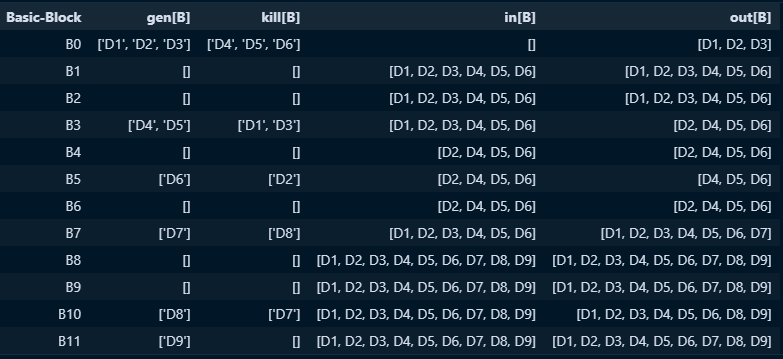
\includegraphics[width=0.8\linewidth]{figures/2_4.png}
    \caption{Final DFA iteration for simple.c}
    \label{2_4}
\end{figure}
\FloatBarrier
where the corresponding definitions are:
\begin{lstlisting}[language=Json]
{
  "D1": ["i", "int i = 0;"],
  "D2": ["x", "int x = 5;"],
  "D3": ["y", "int y = -1;"],
  "D4": ["i", "i = i + 1;"],
  "D5": ["y", "y = i + x;"],
  "D6": ["x", "x = i;"],
  "D7": ["j", "int j = 0;"],
  "D8": ["j", "j++;"],
  "D9": ["z", "int z = j + y;"]
}
\end{lstlisting}

\subsection{Multiple Reaching Definition Identification based on in[B] and out[B] sets}
For each block, using in[B] and out[B] we can tell if some variable has
multiple reaching definitions at a point, by checking if there are multiple
defintions reaching that block for some of its variables. For example, in block
B7, we see that the in[B7] set contains D1 and D4 for variable i, indicating
that at the start of block B7, variable i can have two possible definitions
reaching it: the initial definition (D1) and the updated definition from within
the loop (D4). This indicates that there are multiple paths in the program that
can lead to block B7, each with a different value for i.

For \texttt{simple.c}, the blocks with multiple reaching definitions are:
\begin{lstlisting}[language=Json]
{"B1":{"i":["D1","D4"],"x":["D2","D6"],"y":["D3","D5"]},
 "B2":{"i":["D1","D4"],"x":["D2","D6"],"y":["D3","D5"]},
 "B3":{"i":["D1","D4"],"x":["D2","D6"],"y":["D3","D5"]},
 "B4":{"x":["D2","D6"]},
 "B5":{"x":["D2","D6"]},
 "B6":{"x":["D2","D6"]},
 "B7":{"i":["D1","D4"],"x":["D2","D6"],"y":["D3","D5"]},
 "B8":{"i":["D1","D4"],"x":["D2","D6"],"y":["D3","D5"],"j":["D7","D8"]},
 "B9":{"i":["D1","D4"],"x":["D2","D6"],"y":["D3","D5"],"j":["D7","D8"]},
 "B10":{"i":["D1","D4"],"x":["D2","D6"],"y":["D3","D5"],"j":["D7","D8"]},
 "B11":{"i":["D1","D4"],"x":["D2","D6"],"y":["D3","D5"],"j":["D7","D8"]}
}
\end{lstlisting}

\section{Results and Analysis}

We run the analysis on the three non-trivial C programs mentioned earlier. The
results are stored on the Github repository for this lab.

The cyclomatic complexities for the three programs are shown in
Table~\ref{table:cc_metrics}.

\begin{table}[!ht]
    \centering
    \begin{tabular}{lccc}
        \hline
        \textbf{Program}           & \textbf{E} & \textbf{N} & \textbf{CC} \\
        \hline
        \texttt{dft.c}             & 92         & 73         & 21          \\
        \texttt{integration.c}     & 179        & 147        & 34          \\
        \texttt{labyrinth\_game.c} & 271        & 201        & 72          \\
        \hline
    \end{tabular}
    \caption{CC metrics for the chosen C program.}
    \label{table:cc_metrics}
\end{table}

The iterations for the Reaching Definitions Analysis for these programs are
provided in the Github repository. Some interesting observations are as
follows:

Fig~\ref{2_5} shows the cyclomatic complexity vs (program, LOC) for the three
programs. We observe that as the lines of code increase, the cyclomatic
complexity also tends to increase, indicating more complex control flow in
larger programs.
\begin{figure}[!ht]
    \centering
    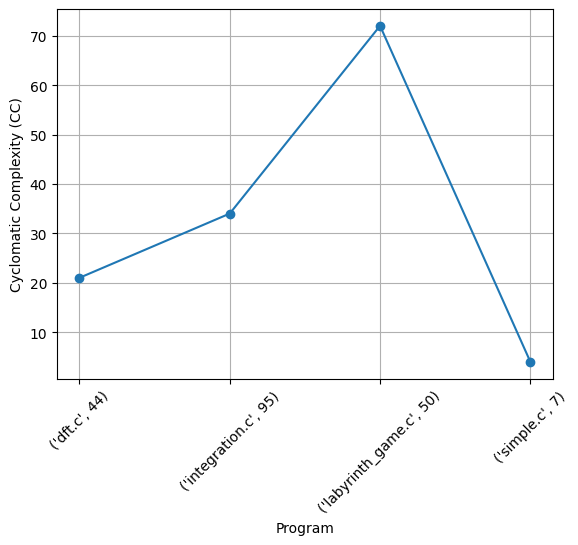
\includegraphics[width=0.5\linewidth]{figures/2_5.png}
    \caption{CC vs program}
    \label{2_5}
\end{figure}

We then plot in the following graphs, the number of changes in In[B] and Out[B]
sets per iteration for the four programs (Fig~\ref{2_6}, Fig~\ref{2_7},
Fig~\ref{2_8} and, Fig~\ref{2_9}).

\begin{figure}[!ht]
    \centering
    \begin{minipage}{0.49\linewidth}
        \centering
        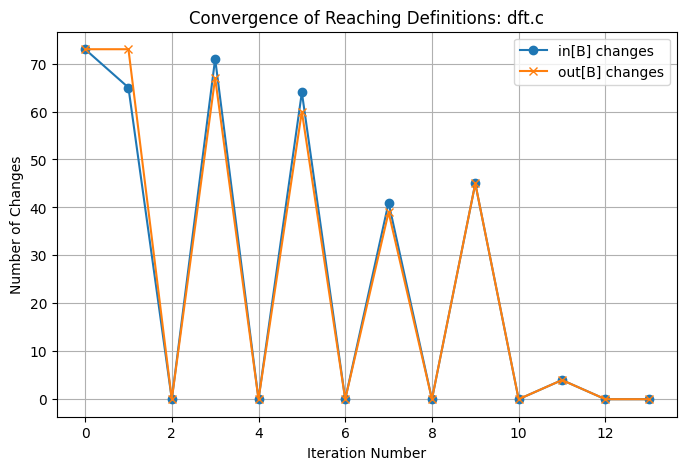
\includegraphics[width=\linewidth]{figures/2_6.png}
        \caption{\texttt{dft.c}: Changes in in[B] and out[B] per iteration}
        \label{2_6}
    \end{minipage}
    \hfill
    \begin{minipage}{0.49\linewidth}
        \centering
        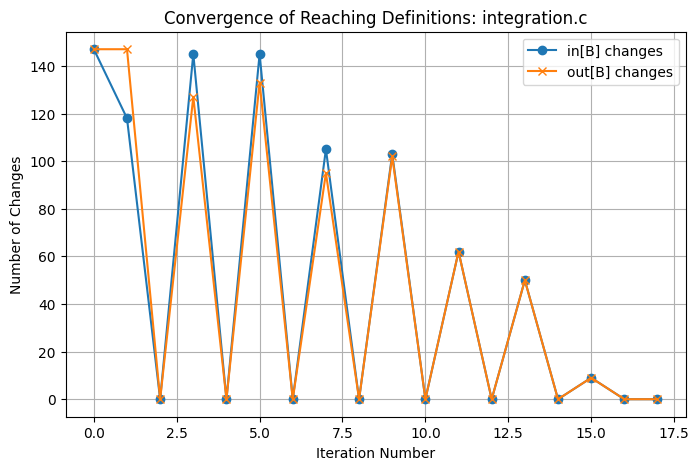
\includegraphics[width=\linewidth]{figures/2_7.png}
        \caption{\texttt{integration.c}: Changes in in[B] and out[B] per iteration}
        \label{2_7}
    \end{minipage}
\end{figure}
\begin{figure}[!ht]
    \centering
    \begin{minipage}{0.49\linewidth}
        \centering
        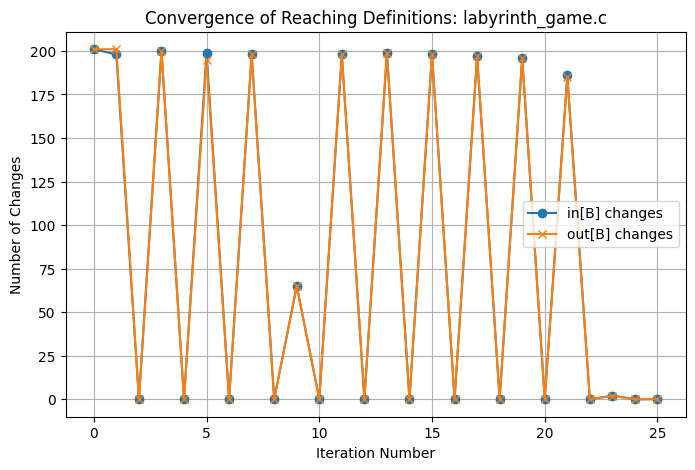
\includegraphics[width=\linewidth]{figures/2_8.png}
        \caption{\texttt{labyrinth\_game.c}: Changes in in[B] and out[B] per iteration}
        \label{2_8}
    \end{minipage}
    \hfill
    \begin{minipage}{0.49\linewidth}
        \centering
        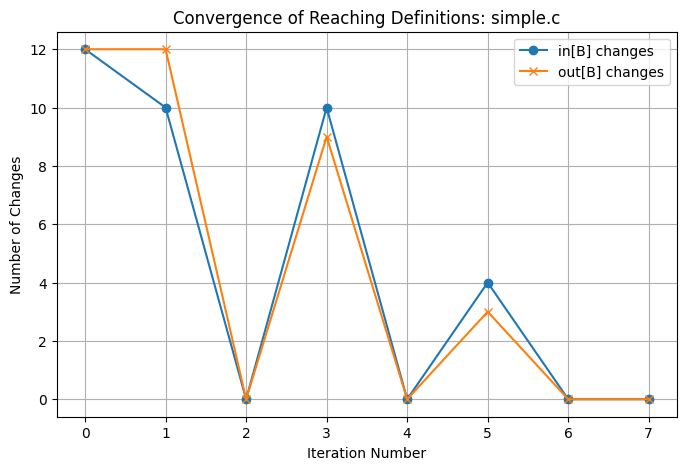
\includegraphics[width=\linewidth]{figures/2_9.png}
        \caption{\texttt{simple.c}: Changes in in[B] and out[B] per iteration}
        \label{2_9}
    \end{minipage}
\end{figure}

We observe that in all four programs, overall the number of changes decreases
with each iteration, indicating convergence of the analysis. However, the
number of changes are alternating between some decreasing value and zero. This
alternating pattern of changes in in[B] and out[B] occurs due to the forward
propagation of reaching definitions. In each iteration, a block's in[B] is
updated from the out[B] sets of its predecessors, and then its out[B] is
updated based on its in[B] and its gen/kill sets. Therefore, a change in out[B]
in one iteration triggers a change in successor in[B] in the next iteration,
and so on, producing a wave-like alternation until the analysis converges.

\section{Discussion and Conclusion}

In this lab, we implemented and understand the principles of Reaching
Definitions Analysis, by constructing CFGs and applying data flow equations to
chosen C programs in increasing complexity. The analysis of the four programs,
from the simple simple.c to the more complex labyrinth\_game.c, showed the
correctness and scalability of our custom \texttt{CFGMaker1000}.

Through constructing the control flow graph and performing reaching definitions analysis, we were able to identify, for each basic block, the definitions of variables that may reach it. The results clearly show that multiple definitions can reach the same block for a given variable, depending on the path taken through the program. This analysis reveals all possible definitions of variables that can be in effect at a program point, showing the effect of control flow and multiple execution paths. This information is useful for compiler level optimzations such as constant propagation, and dead code elimination, since we can determine at compile time if some variable has a single definition or multiple definitions at some point.

\bibliographystyle{IEEEtran}   % or any style you prefer
\nocite{*}
\bibliography{chapters/refs7}           % specific bib file for this chapter
